
\subsection{Supervised methods: machine learning} \label{supervised}

Machine learning techniques are often used when performing a metabolic fingerprinting experiment. It focuses on the construction of algorithms that can learn from and make predictions on data, through building a model from sample inputs. In order to build a predictive model, a set of training data must be provided, and the learner algorithm must have the ability to generalize from its experience, by performing accurate predictions on new, unseen examples. 

In machine learning, tabular data is the most common way of representing the data. It consists in a data table with rows representing the different samples, or X, and a single or multi-column property, or y, that is known for each example (\autoref{tabular_data}). The properties are usually the interesting facts of the examples. When properties are of continuous nature it is called a regression approach, whereas if they are of discrete nature it is called a classification approach \citep{varmuza2009introduction}. The general workflow of a machine learning approach is represented in \autoref{ml_workflow}.

\begin{figure}[!htb]
	\centering
	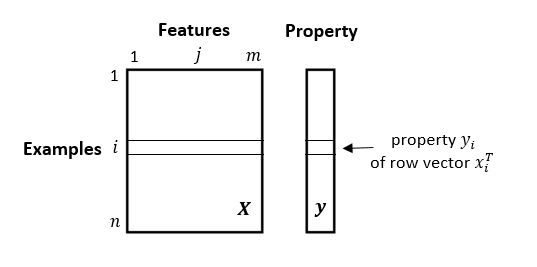
\includegraphics[width=0.6\linewidth]{Imagens/tabular_data}
	\caption{Graphical representation of tabular data used in a machine learning approach, including feature matrix X and a property vector y.}
	\label{tabular_data}
\end{figure}



Among the most popular supervised methods for classification are: \acrfull{plsda}, \acrfull{lda}, \acrfull{simca} and Decision trees. Methods for regression tasks include \acrfull{plsr} and Regression trees. Methods such as \acrfull{knn}, \acrfull{svm}, \acrfull{ann} and Random Forests can be used for both classification and regression tasks.

\acrfull{pls} is a method to relate a matrix X of independent variables to a vector y or to a matrix Y of dependent variables. In the model structure of \gls{plsr}, the X-data is first transformed into a set of intermediate linear latent variables (components). Since it is a linear method, the final latent variable that predicts the modeled property, y, is a linear combination of the original variables. During model development, a relatively small number of \gls{pls} components are calculated, and it is the number of such components that determines the complexity of the model, which can be optimized for high prediction performance. \gls{plsda} is a variant used when the Y is categorical \citep{varmuza2009introduction}.

\begin{figure}
	\centering
	\includegraphics[width=0.85\linewidth]{Imagens/ml_workflow}
	\caption{General workflow of a machine learning approach.}
	\label{ml_workflow}
\end{figure}

\gls{lda} attempts to find a linear combination of features (latent variable) that characterizes or separates two or more classes of objects or events. The resulting combination is commonly used as a linear classifier. The representation of a \gls{lda} model consists of statistical properties of the data, which are calculated for each class and then used to make predictions. For a single input variable, $ x $, these properties are the mean and the variance of the variable for each class, whereas for multiple variables the properties consist in the means and covariance matrix. This method assumes a Gaussian distribution of the data and that each attribute has the same variance. It is closely related to \gls{pca}, although \gls{pca} does not take into consideration the underlying class structure, being sometimes used for data dimensionality reduction \citep{martinez2001pca}.

The \gls{simca} method is based on disjoint principal component models. The idea is to describe the multivariate data structure of each group separately in a reduced space using \gls{pca}. The special feature of this method, is that \gls{pca} is applied to each group separately and also the number of principal components is selected individually and not jointly for all groups.  Due to the use of \gls{pca}, this approach works even for high-dimensional data with rather a small number of samples, whereas methods like \gls{lda} can become unstable under such conditions. In addition to the group assignment for new objects, \gls{simca} also provides information about the relevance of different variables to the classification, or measures of separation \citep{varmuza2009introduction}.

Decision trees consist in a flowchart-like structure in which internal nodes represent the test on an attribute, the branches represent the outcome of the test and the leaves represent a class label. The learning phase is done by splitting the source set into subsets based on an attribute value test, repeating this process in a recursive manner until the subset at a node has the same value of the target variable, or when splitting no longer adds value to the predictions. When the target variable is of discrete nature it is called a classification tree, whereas when the target variable is of continuous nature it is called a regression tree. A Random Forest classifier builds a large collection of uncorrelated trees, and then averages them to improve the classification rate. It uses the bagging method which helps to reduce variance and corrects the decision's tree habit of overfitting to their training set \citep{friedman2009elements}.

In contrast to the already mentioned machine learning methods, the \gls{knn} method does not require a model to be fit. It is a type of lazy learning method, where the function is only approximated locally and all computation is deferred until classification. For \gls{knn} classification, the task is to predict the class membership of a new object $ x $. Using, for instance, the Euclidean distance measure, the k-nearest neighbors (of the training data) to $ x $ are determined. The neighbors are found by calculating the distances between the new object and all objects in the training set. This method has the advantage of neither requiring linearly separable groups nor compact clusters for the groups, being easily applied to multi-class problems \citep{varmuza2009introduction}.

Given a set of training examples and two possible categories for each example, the \gls{svm} algorithm builds a model capable of assigning examples to one of the two categories, making it a non-probabilistic binary linear classifier. It produces linear boundaries between object groups in a transformed space of the $ x $-variables, usually of much higher dimension than the original $ x $-space. These class boundaries are constructed to maximize the margin between the groups. New examples are then mapped into that same space and predicted to belong to a category based on which side of the decision boundary they fall \citep{varmuza2009introduction}.

In \gls{ann}s, the central idea is to extract linear combinations of the inputs as derived features, and then model the target as a nonlinear function of these features. An \gls{ann} is a two-stage regression or classification model, typically represented by a network diagram, where neural units are interconnected. This network usually has three layers, consisting in an input layer, an hidden layer and an output layer. The input data goes into the first layer, the hidden layer nodes do some calculations and then the output is gathered from the last layer. The links between different neural units can be enforcing or inhibitory in their effect on the activation state of connected neural units, usually through a limiting (threshold) function \citep{friedman2009elements}.

Some of these (and other) machine learning methods used in spectral data analysis studies available in the literature are listed on the fifth column of \autoref{spectroscopies}.





